\documentclass[twocolumn]{article}


\usepackage{fullpage}
\usepackage{amsmath}
\usepackage{amssymb}
\usepackage{graphicx}
\usepackage{float}
\usepackage{natbib}
\usepackage[capitalise,noabbrev]{cleveref}
\usepackage{enumitem}
\usepackage{multirow}
\usepackage{breqn}
%\usepackage{cite}

\newcommand{\img}[1]{\includegraphics[width=3in]{#1}}
\newcommand{\ep}{\varepsilon}
\newcommand{\RR}{\mathbb{R}}

\begin{document}
	
\twocolumn[{
	\centering
	\LARGE Bayesian Marginal Likelihood Estimation Using\\ Iterative Kernel Density Estimation\\[1.0em]
	\large Taylor McKenzie\\[1.0em]
}]

\begin{abstract}
	Bayesian statistics provides a very general, well-founded, and intuitive framework for model selection. Any exclusive models that permit a proper posterior distribution can be compared via Bayes' factors, and the probability that any given model from a set of potential models is correct can be calculated. However, it can be hard to estimate Bayes' factors due to difficulties in computing a model's marginal likelihood. Methods have been developed to make this problem computationally feasible for models that can be fit with Gibbs or Metropolis-Hastings samplers \citep{Chib,ChibJeliazkov}, and more general methods have been developed that are suitable for moderately-sized models applied to medium to large datasets. Unfortunately, existing methods do not perform well for large models applied to small or medium samples. This research develops a general algorithm to estimate marginal likelihood and, by extension, Bayes' factors using iterative kernel density estimation. While this technique is widely applicable and can be used with large or small models and data alike, it specifically fills a gap in existing methods by addressing models with many parameters and relatively limited data. The developed model selection method is applied to production data to select between three stochastic frontier models that assume different forms of the production function: log-linear, translog, and a flexible form derived from a Gaussian process.
\end{abstract}

\section{Introduction}

Model selection serves an important role in many statistical analyses. There are a host of model selection techniques available to researchers whose applicability and efficacy depends on the model, estimation framework, and characteristics of the data. Methods available in classical statistics tend to rely on asymptotic results and therefore require larger sample sizes. Likewise, model selection methods used in machine learning, such as cross-validation, also tend to be data intensive. Bayesian model selection, on the other hand, is capable of testing between any exclusive models for which a likelihood function and priors over the parameters can be specified, regardless of sample size. In this framework, the probability that any given model from a set of exclusive models is the true model can be calculated through computation of the model's marginal likelihood. Unfortunately, marginal likelihood can be difficult to compute, giving rise to many estimation techniques for a variety of situations. Some techniques, like Laplace's method, perform well in small to moderate sized models with large datasets. Schwarz Bayesian Information Criterion can be used to approximate marginal likelihood and perform well for large and small models alike, but rely on large sample sizes to justify approximations. Other methods, such as bridge sampling, perform well for small- to moderately-sized models and for all sample sizes, but can encounter numerical issues in large models. To the best of my knowledge, no existing method adequately addresses marginal likelihood estimation of large models applied to relatively small datasets. This paper presents method that uses iterative sampling of conditional posterior distributions and kernel density estimation (KDE) to arrive at an estimate of marginal likelihood that is consistent even for large models and small datasets.

I begin with a review of relevant literature, including existing model selection techniques, methods for KDE, and a summary of Markov Chain Monte Carlo, a widely used method of estimating Bayesian models. I then present the iterative KDE algorithm and explain why it is applicable for models in which others methods are not. Simulation results for several models follows, showing that iterative KDE produces consistent estimates of marginal likelihood. Finally, I present three stochastic frontier models and a relatively limited dataset and select between them using marginal likelihoods calculated with iterative KDE. One of the models uses a flexible functional form of the production function derived from a Gaussian process. This model has many parameters, so existing methods would not be suitable for marginal likelihood estimation and the suitability of iterative KDE is demonstrated.

\section{Literature Review}

\subsection{Model Selection}
\label{sec:ModelSelection}
%Citations here: 
%Classical: Greene, Morgan (LR Test), Akaike, Schwarz (SBIC), Bollen (performance of AIC/SBIC in small samples)
%Cross-validation: Allen, Golub, Kohavi (machine learning), Arlot (survey of methods)
%Bayeisan: Chib, Chib & Jeliazkov, Kass & Raftery (Bayes' factor), George (mixed model selection), Berger (?)

When building statistical models, researchers face a number of difficult decisions. Which variables should be included in the analysis? What functional form should the model assume? Should a parametric, non-parametric, or machine learning approach be taken? Many statistical model selection methods have been proposed to formally evaluate the validity of modeling decisions. This subsection presents a broad overview of those methods, their applicability, and relative advantages.

Model selection techniques can largely be categorized into within-sample and cross-validation methods. Within-sample model selection evaluates how well the model fits the data that were used to estimate parameters of the model \citep{Greene}. Cross-validation, on the other hand, splits the sample into two parts: one used for estimating parameters, called the training set, and another used for evaluating the model's performance, called the validation set \citep{Arlot}. Cross-validation is often used when over-fitting is a concern. Over-fitting can occur when a flexible model specification is used, which can cause the estimated model to fit the training set very well but have difficulties making accurate predictions outside of the training set. However, cross-validation can be data intensive and less suitable to smaller datasets. Cross-validation methods have grown in popularity, especially among machine-learning methods, which tend to use very flexible specifications and are typically applied to large datasets.\footnote{For more examples of cross-validation applications, see \cite{Allen}, \cite{Golub}, and \cite{Kohavi}.}

Economic studies often use within-sample model selection methods, often because data tend to be relatively limited \citep{Greene}. For classical (i.e., frequentist) statistical models, selection techniques tend to be based on the likelihood of the data given parameter estimates.\footnote{While $R^2$ and adjusted $R^2$ are often used to inform model selection, they do not lend themselves well to formal hypothesis testing because distributions relating $R^2$ between two models is not generally known, even asymptotically.} Likelihood ratio tests, which subsume $Z$-, $F$- and $\chi^2$ tests in linear models, compare likelihoods of a null model and alternative model nested in the null model, then conduct a formal hypothesis test between the two models \citep{Morgan}. For non-nested models, information criteria are often used for model selection. Commonly used information criteria include Akaike Information Criterion (AIC), described in \cite{Akaike}, and Schwarz-Bayesian Information Criterion (SBIC), described in \cite{Schwarz}. Both AIC and SBIC take into account likelihood of the data given parameter estimates and the number of parameters in the model, and SBIC places greater penalty on additional parameters. SBIC can be used to approximate the posterior model probability, described in greater detail later in this subsection. Model selection in classical statistics, including use of AIC and SBIC, tend to rely on asymptotic results and can therefore be less applicable to smaller samples.

For Bayesian statistical models, which are the focus of this research, model selection has traditionally been conducted via posterior model probabilities. In general, for a set of exclusive models $\{M_1, ..., M_K\}$ and data $y$, the probability that model $M_k$ is the true model is given by
\begin{equation}
	\Pr(M_k|y) = \frac{m(y|M_k)p(M_k)}{\sum_{j=1}^K m(y|M_j)p(M_j)},
\end{equation}
where $m(y|M_j)$ is the marginal likelihood of model $M_j$ and $p(M_j)$ is the prior probability that model $M_j$ is the true model, specified by the researcher \citep{KassRaftery}. These model probabilities can either be used to select a single best-performing model or to perform Bayesian model averaging, which weights predictions from each model by their respective model probabilities to form a meta-prediction. The marginal likelihood of model $M_j$ is defined as
\begin{equation}
m(y|M_j) = \int f(y|\theta_j, M_j) p(\theta_j|M_j)d\theta_j,
\end{equation}
where $f(y|\theta_j, M_j)$ is the likelihood of the data in model $M_j$ given parameters $\theta_j$, and $p(\theta_j|M_j)$ are prior assumptions over parameters $\theta_j$ in model $M_j$, defined by the researcher. As noted by \cite{KassRaftery}, this integral is taken over the entire parameter space; as the number of parameters in the model grows, direct integration of marginal likelihood becomes computationally infeasible due to the curse of dimensionality.

Fortunately, methods have been developed to estimate marginal likelihood in a computationally efficient way when Gibbs or Metropolis-Hastings (M-H) samplers are used to draw samples from posterior distributions of parameters. \cite{Chib} notes that marginal likelihood can be written as 
\begin{equation}
	\label{eq:MLChib}
	m(y|M_j) = \frac{f(y|\theta_j, M_j)p(\theta_j|M_j)}{p(\theta_j|y, M_j)},
\end{equation}
where $p(\theta_j|y, M_j)$ is the posterior density of parameters $\theta_j$. First, one can see from this relationship that the inclusion of additional parameters does not come without cost to marginal likelihood. When priors are reasonably diffuse, values of the prior density $p(\theta_j|M_j)$ for each individual parameter tend to be less than one, decreasing marginal likelihood. Additionally, as discussed in \cref{sec:Theory}, posterior density can be viewed as a measure of redundancy of parameters; marginal likelihood will be further penalized if parameters serve similar purposes in the model. If the additional predictive power offered by the inclusion of another parameter does not outweigh its cost through the prior density, there will be a net decrease in marginal likelihood. Second, while the likelihood $f(y|\theta_j, M_j)$ and prior density $p(\theta_j|M_j)$ are easily calculable, the posterior density can be difficult to calculate in general. However, \cite{Chib} derived an estimate of posterior probabilities, and marginal likelihood by extension, when using a Gibbs sampler. \cite{ChibJeliazkov} extended this work to estimate marginal likelihood under a M-H sampler.

\cite{KassRaftery} detail several methods for estimating marginal likelihood when Gibbs or M-H sampling are not used. Laplace's method forms a second-order approximation of the posterior density, with which marginal likelihood can be estimated. For sufficiently large numbers of observations, Laplace's method is both accurate and computationally efficient; however, accuracy is severely degraded when the number of observations is less than $5\times d$, where $d$ is the number of parameters in the model \citep{Slate}. While this requirement tends to be met by standard models and datasets, it can present issues with more flexible models, such as those presented in \cref{sec:SF}. Further, even when requirements of Laplace's method are met, other estimators, such as those in \cite{Chib}, can have lower variance. SBIC, mentioned previously, can also be used to obtain consistent estimates of marginal likelihood, but are also less efficient for small sample sizes \citep{Bollen}. Other methods focus on using Monte Carlo integration to estimate marginal likelihood. Unfortunately, relatively simple Monte Carlo integration, such as the harmonic mean estimator
\begin{equation}
	\hat{m}(y|M_j) = \left(\frac{1}{S} \sum_{s=1}^S \frac{1}{f(y|\theta_j^{[s]}, M_j)}\right)^{-1},
\end{equation}
where $\theta_j^{[s]}$ is the $s$th sample from the posterior of model $M_j$, is not stable because inverse likelihood does not have finite variance \citep{NewtonRaferty}. This problem can be circumvented via use of importance sampling or Gaussian quadrature, but these solutions can be computationally infeasible for models with moderately large numbers of parameters \citep{GenzKass}.

Finally, \cite{MengWong} propose using bridge sampling as a method of approximating marginal likelihood. For moderately-sized models, bridge sampling can produce low variance estimates that outperform many, if not all, of the previously mentioned marginal likelihood estimation techniques. The authors derive and utilize the following identity (model notation is now dropped for simplicity):
\begin{equation}
	\label{eq:bridgeIdentity}
	%m(y|M_j) = \frac{\int p(y|\theta_j, M_j)p(\theta_j|M_j)h_j(\theta_j)g_j(\theta_j) d\theta_j}{\int h_j(\theta_j)g_j(\theta_j)p(\theta_j|y, M_j) d\theta_j},
	m(y) = \frac{\int p(y|\theta)p(\theta)h(\theta)g(\theta) d\theta}{\int h(\theta)g(\theta)p(\theta|y) d\theta},
\end{equation}
where $g$ is the proposal distribution and $h$ is called the bridge function. To approximate the integrals in \cref{eq:bridgeIdentity}, one can draw $N_1$ samples from the posterior distribution $p(\theta|y)$, denoting the $s$th sample $\theta_{y}^{[s]}$, and $N_2$ samples from the proposal distribution $g(\theta)$, denoting the $s$th sample $\theta_{g}^{[s]}$. Then, marginal likelihood can be estimated with
\begin{equation}
	\label{eq:bridgeEstimate}
	\hat{m}(y) = \frac{\frac{1}{N_2}\sum_{s=1}^{N_2} p\left(y|\theta_{g}^{[s]}\right)p\left(\theta_{g}^{[s]}\right)h_j\left(\theta_{g}^{[s]}\right)}{\frac{1}{N_1}\sum_{s=1}^{N_1} h\left(\theta_{y}^{[s]}\right)g\left(\theta_{y}^{[s]}\right)}.
\end{equation}
While choosing the proposal distribution $g$ is relatively straightforward (typically an approximation of the posterior), selecting the bridge function $h$ is more involved. \cite{MengWong} derive an optimal bridge function, given by
\begin{equation}
	\label{eq:bridgeFunction}
	h(\theta) = \left(r_1 p(y|\theta) p(\theta) + r_2 \hat{m}(y) g(\theta)\right)^{-1},
\end{equation}
where $r_1 = N_1 / (N_1 + N_2)$ and $r_2 = N_2 / (N_1 + N_2)$. Note that the marginal likelihood $\hat{m}_y$ appears in $h(\theta)$, and an iterative approach can be used to find the value of the marginal likelihood that satisfies \cref{eq:bridgeEstimate} and \cref{eq:bridgeFunction}. While this relationship holds in theory, problems can arise in practice due to limitations in machine precision. Specifically, computers will round arithmetic operations to the next largest multiple of machine precision because arbitrarily large decimal expansions cannot be stored on a finite memory machine \citep{MachinePrecision}. Thus, for two real numbers $z_1$ and $z_2$, the product $z_1 z_2$ is computed as $z_1 z_2 (1 + u)$, where $u$ is at most the machine precision.\footnote{Machine precision is typically a very small positive number that varies across data types and computers. Ultimately, memory limitations dictate the lowest machine precision a given computer is capable of.} When the number of parameters in the model is large, several of the distributions in \cref{eq:bridgeEstimate} and \cref{eq:bridgeFunction} can take on very small values. As a result, terms in the the sums in the numerator and denominator of \cref{eq:bridgeEstimate} can take on extreme values, making the absolute difference between the true quotient and computed quotient large.  Since computation of the numerator and denominator involve summing these extreme values, this problem cannot be effectively mediated with numerical methods like log-transformation. These numerical issues can ultimately bias estimates of marginal likelihood, as exemplified in \cref{sec:BridgeSimulation}.

Overall, it can be difficult to accurately estimate marginal likelihood for models with relatively few observations and many parameters using previously established techniques. Kernel density estimation, which to the best of my knowledge has not been used for marginal likelihood estimation, could theoretically be used to estimate the posterior density $p(\theta_j|y, M_j)$ and, by extension, marginal likelihood, as in \cref{eq:MLChib}. However, this method has not been feasible historically due to practical issues with many kernel density estimators, described in greater detail in the following subsection.

\subsection{Kernel Density Estimation}
\label{sec:KDE}
%Citations here:
%Silverman (most density estimation, including standard, adaptive, etc.)
%Portnoy (application of adaptive KDE and some references)
%Beran (adaptive rank estimator)

%Idea for this section: Lay out KDE basics (formula), illustrate weakness (bias in density estimates), state how adaptive KDE fixes.

Distributional approximation arises often in statistical analysis. Researchers will often have a sample of data drawn from an unknown density which they want to approximate, either as a whole or at specific points. Kernel density estimators are a non-parametric method of approximating such densities. Given a sample $x_1, ..., x_N$ where each $x_i\in\RR^k$ for $k\geq1$, a kernel density estimator for a density $f$ at a point $x$ is defined as
\begin{equation}
	\hat{f}_\lambda(x) = \frac{1}{N}\sum_{i=1}^N K_\lambda(x - x_i),
\end{equation}
where $K_\lambda$ is a kernel chosen by the researcher, parameterized by $\lambda$ \citep{SilvermanDE}. A normal distribution is often used as a kernel, so that
\begin{equation}
	K_\lambda(z) = K_H(z) = \det(2\pi H)^{-\frac12} \exp\left(-\frac12 z' H^{-1} z\right).
\end{equation}
The matrix $H\in\RR^{k\times k}$ is called the bandwidth matrix and must be positive definite.\footnote{There are a number of methods that can be used to select the bandwidth matrix. For more reading, see \cite{SilvermanDE}, \cite{Scott}, and \cite{SheatherJones}.}

Unfortunately, standard kernel density estimators such as that presented above can produce biased estimates in finite samples \citep{SilvermanDE}. These estimators tend to underestimate density in high-density regions and overestimate density in low-density regions. Methods like adaptive kernel density estimation have been developed to produce unbiased density estimates in finite samples \citep{Portnoy}. Whereas standard kernel density estimation holds the bandwidth matrix constant over the domain, adaptive kernel density estimators allow bandwidth to vary based on a rule that chooses smaller bandwidths for high-density regions and larger bandwidths for low-density regions.

The curse of dimensionality presents another problem for kernel density estimation in general. Specifically, the number of sample points $N$ needed to achieve acceptable density estimates (that is, the expectation of the estimate is with a neighborhood of its true value) grows as $O\left(N^{-4/(4+d)}\ln(N)\right)$, where $d$ is the number of dimensions \citep{LiuLafferty}. A number of methods have been proposed to mediate the effect of the curse of dimensionality. Central to the methods in this research, if density only needs to be estimated at a small number of points and conditional densities can be efficiently sampled, the definition of conditional probability can be used to break the joint density estimation into $d$ separate univariate density estimations, detailed in \cref{sec:Theory}.

\subsection{Markov Chain Monte Carlo Samplers}
%Citations here:
%Gelfand & Smith (overview)
%Chib & Greenberg (M-H), Geman (Gibbs), Tanner & Wong (data augmentation), Rubin (importance sampling)

As alluded to in \cref{sec:ModelSelection}, in order to estimate Bayesian statistical models and to use Bayesian model selection, one must be able to sample from the posterior distribution of parameters given then data, written $p(\theta|y)$. For some models, the posterior has a known closed form, which can be sampled from directly; however, most models do not permit a closed form, so other sampling methods must be used. Markov Chain Monte Carlo (MCMC) is a simulation algorithm used to draw samples from the posterior distribution even when the exact form of that distribution is unknown \citep{GelfandSmith}. MCMC constructs a Markov chain whose steady-state distribution is the posterior distribution. In practice, the Markov chain is initialized at a specified point, a given number of steps called ``warmup iterations'' are taken to bring the Markov chain sufficiently close to its steady-state, at which point additional steps called ``sampling iterations'' will produce samples from the posterior distribution.

Gibbs and Metropolis-Hastings samplers are two early-developed and widely-used MCMC techniques. Gibbs sampling can be used when the researcher knows the conditional posterior distributions of each parameter given every other parameter (i.e., $p(\theta_i|\theta_{-i}, y)$ for each $i$, where $\theta_{-i}$ represents all parameters in $\theta$ except for $\theta_i$). Metropolis-Hastings, which draws new samples from a proposal distribution and accepts or rejects those based on value of the posterior, does not require knowledge of these conditional distributions and can therefore be more widely applicable. Unfortunately, both Gibbs and Metropolis-Hastings sampling produce posterior samples that have a high degree of autocorrelation. As a result, the information in a posterior sample grows relatively slowly as the number of sampling iterations increases. The notion of ``effective sample size'' has been introduced to estimate the number of ostensibly independent draws obtained from the posterior distribution \citep{Lenth}. Estimates and functions of estimated parameters, such as marginal likelihood, will have lower variance as the effective sample size increases.

Many techniques have been developed to lower autocorrelation within MCMC samples. Some of these solutions, such as \cite{Gilks}, extend Gibbs and Metropolis-Hastings samplers. Hamiltonian Monte Carlo (HMC) presents another solution to the autocorrelation problem and is distinct from Gibbs and Metropolis-Hastings. In general, HMC follows a particle through the parameter space, and the velocity of the particle varies with the gradient of the posterior distribution \citep{Girolami}. A central parameter in HMC is the number of steps a particle is allowed to take before its value is recorded as a sample from the posterior. The effectiveness of HMC depends on the step size chosen by the researcher. No U-Turn Sampling (NUTS) avoids arbitrary selection of the number of steps by stopping the particle and recording its value once it turns back towards its initial position \citep{NUTS}. NUTS has been shown to exhibit far less autocorrelation than many other MCMC algorithms, increasing the proportion of effective samples in a given sampling of the posterior distribution. NUTS has been implemented in the Stan software package, which is utilized by this research \citep{rstan}.

\section{Theory and Method}
\label{sec:Theory}

As mentioned previously, models estimated in the Bayesian framework can be compared via their marginal likelihoods. For two models $M_j$ and $M_k$, the relative goodness-of-fit of $M_k$ over $M_j$, called the Bayes' factor, is the ratio of the marginal likelihoods of each model, expressed as
\begin{equation}
	\frac{m(y|M_k)}{m(y|M_j)}.
\end{equation}
The marginal likelihood of $M_k$ can be written as
\begin{equation}
	m(y|M_k) = \frac{f(y|\theta, M_k)p(\theta|M_k)}{p(\theta|y, M_k)},
\end{equation}
where $\theta$ are parameters of the model, $f(y|\theta, M_k)$ is the likelihood of the data, $p(\theta|M_k)$ is the value of the prior density, and $p(\theta|y, M_k)$ is the posterior density. As noted by \cite{Chib}, this identity holds for each $\theta$, and while the values of the likelihood and prior density are typically known (because they are specified to estimate the model), the value of the posterior density is usually unknown, motivating the development of many Markov Chain Monte Carlo (MCMC) techniques to sample from the posterior distribution. In practice, the marginal likelihood must be estimated at a point $\theta^*$ via estimation of the posterior density. As noted by \cite{Chib}, using $\theta^*$ from a high-density region of the posterior can reduce the variance of marginal likelihood estimates.

While a number of methods have been developed to estimate the value of the posterior density in specific cases, a general approach is to use kernel density estimation (KDE), which can be used to construct and estimate values of a density function from samples of a random variable. Since all MCMC methods produce samples of $\theta|y, M_k$, this method can be used for any MCMC algorithm. However, there are two fundamental issues that complicate this approach. First, many standard KDE procedures produce biased estimates of the density function, systematically underestimating values in high-density regions and overestimating values in low-density regions \citep{SilvermanDE}. Fortunately, as detailed in \cref{sec:KDE}, this is easily remedied via use of more sophisticated KDE methods, such as adaptive KDE.

The other issue complicating the use of KDE to estimate posterior densities is based in the curse of dimensionality. In practice, the posterior density is often a function of several parameters, and KDE becomes less reliable as the number of dimensions grows large and is often completely infeasible for more than five dimensions. To illustrate a solution, first denote the parameter vector as $\theta = (\theta_1, \theta_2, ..., \theta_P)',$ where $P$ is the total number of parameters. Using the definition of conditional probability (and now omitting conditioning on model $M_k$), we can write the marginal likelihood as
\begin{subequations}
\begin{align}
	p(\theta|y)
	&= p(\theta_1, ..., \theta_P|y) \\
	&= p(\theta_1|\theta_2, ..., \theta_P, y)\times p(\theta_2, ..., \theta_P|y) \\
	&= p(\theta_1|\theta_2, ..., \theta_P, y)\times p(\theta_2|\theta_3, ..., \theta_P, y) \\ &\qquad\times p(\theta_3, ..., \theta_P|y) \\
	&= ... \\
	&= p(\theta_1|\theta_2, ..., \theta_P, y)\times p(\theta_2|\theta_3, ..., \theta_P, y)\\ &\qquad\times ...\times p(\theta_P|y).
\end{align}
\end{subequations}
So, the value of the posterior density can be consistently estimated using the following procedure, from here on referred to as iterative KDE:
\begin{enumerate}[noitemsep]
	\item Draw samples of $\theta|y$ using an MCMC algorithm.
	\item Choose $\theta^*$ from a high-density region of $\theta|y$, such as the sample mean or maximum a posteriori.
	\item Estimate the log-density of $\theta_P|y$ at $\theta_P^*$ using adaptive KDE, denoting that value $\ln \hat{p}(\theta_P^*|y)$.
	\item For each $i$ from $P-1, ..., 1$:
		\begin{enumerate}
			\item Re-estimate the model, setting $(\theta_{i+1}, ..., \theta_P) = (\theta_{i+1}^*, ..., \theta_P^*)$, to obtain draws of $(\theta_1, ..., \theta_i)|(\theta_{i+1}^*, ..., \theta_P^*), y$.
			\item Estimate the log-density of $\theta_i|\theta_{i+1}^*, ..., \theta_P^*, y$ at $\theta_i^*$ using adaptive KDE, denoting that value $\ln \hat{p}(\theta_i^*|\theta_{i+1}^*, ..., \theta_P^*, y)$.
		\end{enumerate}
	\item Find the sum of each of the estimated partial log-densities to arrive at an estimate for the overall log-posterior density, denoted $\ln \hat{p}(\theta^*|y)$.
\end{enumerate}

Before moving on, it can be useful to note this iterative formulation sheds some insight on the interpretation of the log posterior density. We can think of $p(\theta_i|\theta_{i+1}^*, ..., \theta_P^*, y)$ as being inversely related to additional information provided by $\theta_i$ to the model, given values of parameters $\theta_{i+1}^*, ..., \theta_P^*$. If the value of $p(\theta_i|\theta_{i+1}^*, ..., \theta_P^*, y)$ is relatively large, then $\theta_i$ provides relatively little information beyond that provided by $\theta_{i+1}, ..., \theta_P$. Thus, if the value of the posterior density as whole is low, there relatively little redundancy between parameters in the model. This serves as yet another penalty of adding parameters to a model, on top of penalties coming from prior assumptions as previously mentioned.

This iterative formulation is by no means novel (a similar formulation was used in \cite{Chib} and \cite{ChibJeliazkov} for Gibbs and Metropolis-Hastings (M-H) samplers, respectively), nor is the method to estimate densities. However, this technique does have a few advantages that together make it distinct from other model selection methods. First, like Laplace's method, bridge sampling, and related methods, iterative KDE enables model selection for any model which has a likelihood function and for which priors over parameters can be specified. Specifically, this technique is not limited to comparing nested models or models estimable with Gibbs or M-H sampling. Second, like bridge sampling, iterative KDE performs well in small- and medium-sized samples. Third, and unlike bridge sampling, Laplace's method, and information criterion, iterative KDE can perform well in large models with relatively limited data and does not suffer from numerical issues. Specifically, individual densities used to compute log marginal likelihood in iterative KDE are typically not extreme, and all densities can be kept in log terms through the entire calculation, drastically reducing the potential for issues related to machine precision to arise.

\section{Simulation Results}

This section presents simulation results to first illustrate the unbiased, lower-variance estimates of marginal likelihood produced by iterative KDE compared with the method proposed by \cite{Chib} to estimate marginal likelihood using Gibbs sampling. The proposed methodology relies on use of a the No U-Turn Sampler (NUTS), which provides better mixing than traditional samplers in order to reduce variance of marginal likelihood estimates. Second, this section presents simulations comparing models that are difficult or impossible to estimate and compare using previously developed techniques to illustrate the generality of iterative KDE.

\subsection{Multivariate Normal Linear Model, Comparison With Gibbs Sampling}

% latex table generated in R 3.5.0 by xtable 1.8-3 package
% Fri Oct 12 17:08:17 2018
\begin{table*}
\centering
\begin{tabular}{l|c|c|c|c}
   &  &  &  & Mean Test \\ 
  Model & \# Trials & Gibbs/Chib & Iterative KDE & $p$-value \\ 
   \hline
\hline
\multirow{3}{*}{Multivariate Linear} & \multirow{3}{*}{500} & -481.353 & -481.348 & \multirow{3}{*}{0.493} \\ 
   &  & (0.154) & (0.078) &  \\ 
   &  & Iter = 5,000 & Iter = 5,000 &  \\ 
   \hline
\multirow{3}{*}{Probit} & \multirow{3}{*}{500} & -23.991 & -23.989 & \multirow{3}{*}{0.446} \\ 
   &  & (0.04) & (0.057) &  \\ 
   &  & Iter = 50,000 & Iter = 5,000 &  \\ 
   \hline
\end{tabular}
\caption{Comparison of Gibbs and Iterative KDE} 
\label{tab:MVN-Probit}
\end{table*}


These simulations begin with a standard multivariate linear model with independent, identically-distributed (iid) normal errors. This model takes the form
\begin{subequations}
\begin{align}
	y &= X\beta + \ep \\
	\ep &\sim iid \mbox{ }N(0, \sigma^2). 
\end{align}
\end{subequations}
The matrix of independent variable data, $X$, contained 100 rows (observations) three columns: one constant columns of ones and two independent columns of uniformly random data in the interval $[-10, 10]$. The parameters of the model were arbitrarily chosen as $\beta = (-2, 5, 3)'$ and $\sigma = 25$. The data was generated once and used repeatedly with a Gibbs sampler and NUTS to produce an empirical distribution of marginal likelihoods for this data and model.

Priors over parameters were chosen so that conditional distributions of parameters could be derived, thereby allowing estimation via Gibbs sampling. Specifically, the priors chosen were
\begin{subequations}
\begin{align}
	\beta &\sim N(0_3, 100\times I_3)\\
	\sigma^2 &\sim \Gamma^{-1}(1, 1).
\end{align}
\end{subequations}
Using these priors, Gibbs sampling of the posterior distribution $\beta, \sigma^2|y, X$ can be achieved via alternative sampling of the conditional distributions
\begin{subequations}
\begin{align}
	\beta|\sigma^2, X, y &\sim N(\mu_\beta, \Sigma_\beta) \\
	\sigma^2|\beta, X, y &\sim \Gamma^{-1}\left(\frac{N}2, \frac{e'e}2 + 1\right),
\end{align}
\end{subequations}
where
\begin{subequations}
\begin{align}
	\Sigma_\beta &= \left(\frac{X'X}{\sigma^2} + \frac1{100}\times I_3\right)^{-1}\\
	\mu_\beta &= \Sigma_\beta\left(\frac{X'y}{\sigma^2}\right)\\
	e &= y - X\beta.
\end{align}
\end{subequations}
Estimation of marginal likelihood from this Gibbs sampler followed the three vector block example from \cite{Chib}. The same model and assumptions were also coded in Stan and marginal likelihood was estimated using the previously described methodology. Each method used 500 warm-up and 5,000 sampling iterations and each was run 500 times to sample the distribution of marginal likelihoods.

The results of this simulation can be found in the first row of \Cref{tab:MVN-Probit}. The Gibbs and Iterative KDE columns show the sample mean of marginal likelihood and standard deviation in parentheses. The sample means from each method are approximately equal, and a mean equality test with the alternative hypothesis that the mean marginal likelihoods were not equal yielded a $p$-value of 0.493, indicating that the data do not suggest the true means are different at the 10\% level of significance. Since the method used in \cite{Chib} yields unbiased estimates of marginal likelihood, this finding provides evidence that the proposed method also produces an unbiased estimator of marginal likelihood.

Further, the standard deviation of the Gibbs sampling based method was 0.154 while that of the iterative KDE method was 0.078. A variance equality test was run, with the alternative hypothesis that the variance of the iterative KDE method was less than that of the Gibbs-based method, and yielded a very small $p$-value (below machine precision), implying the data provides evidence that the proposed method has lower variance than the Gibbs-based method for similar numbers of sampling iterations. As mentioned before, this is likely due to the fact that NUTS provides better mixing and therefore greater effective sample size from the posterior distribution, thereby reducing the variance of marginal likelihood estimates. However, the iterative KDE method took around three times as long to run as the Gibbs sampling method on average. Another simulation was run, using 500 warm-up and 2,500 sampling iterations for NUTS and 1,000 warm-up and 15,000 sampling iterations for Gibbs sampling to make computational runtimes approximately equivalent,\footnote{Numbers of iterations were chosen to make Gibbs sampling runtimes slightly longer than NUTS to give the former method the benefit of the doubt.} and similar results were found. Both methods still had equivalent means at the 10\% level, and while the variance of the iterative KDE method was higher (0.100) and that of the Gibbs-based method was lower (0.146) than the previously presented results, the iterative KDE method still had significantly lower variance. It is important to note that this final result may not generalizable; as the number of parameters increases (especially parameters that can be evaluated in blocks by the Gibbs sampler, like $\beta$), the iterative KDE method will take relatively more time to run compared to the Gibbs-based method because the model must be rerun conditioning on each individual parameter when using iterative KDE.

\subsection{Probit Model, Comparison With Gibbs Sampling}
\label{sec:ProbitGibbs}

Next, the probit model of binary outcomes will be considered. This model has the form
\begin{subequations}
\begin{align}
	z &= X\beta \\
	\Pr(y=1|X) &= \Phi(z) \\
	\Pr(y=0|X) &= 1 - \Phi(z),
\end{align}
\end{subequations}
where $\Phi$ is the cumulative normal distribution. The matrix of independent variable data, $X$, had 100 observations and two columns: one constant column of ones and one column of uniformly distributed random numbers in the interval $[-1, 1]$. The parameter of the model was arbitrarily chosen to be $\beta = (-2, 5)'$. The data and parameters had to be chosen carefully because convergence of the Gibbs sampler can be difficult in the probit model when the latent variable $z$ takes on extreme values (this presents much less of a problem in the Stan implementation of NUTS). The priors of the model were specified as
\begin{align}
	\beta &\sim N(0_2, 100 \times I_2).
\end{align}
The sampler and estimates of the marginal likelihood were obtained via the methodology directly described in \cite{Chib}. Each algorithm was again run 500 times to produce empirical distributions of marginal likelihoods.

% latex table generated in R 3.5.1 by xtable 1.8-2 package
% Thu Oct 18 08:44:20 2018
\begin{table*}
\centering
\begin{tabular}{c|c|c|c|c}
   & Iterative &  & IKDE = Chib & Bridge = Chib \\ 
  Chib & KDE & Bridge & $p$-value & $p$-value \\ 
   \hline
\hline
-606.927 & -606.88 & -607.094 & \multirow{2}{*}{0.125} & \multirow{2}{*}{$1.777\times 10^{-13}$} \\ 
  (0.195) & (0.24) & (0.014) &  &  \\ 
   \hline
\end{tabular}
\caption{Comparison of Chib, Iterative KDE, and Bridge Sampling} 
\label{tab:bridge}
\end{table*}


Results of this simulation are shown in the second row of \Cref{tab:MVN-Probit}. Once again, the mean marginal likelihood estimates were not found to be significantly different at the 10\% level. The standard deviation of the iterative KDE method was slightly larger than that of the Gibbs-based method due to differences in the numbers of sampling iterations used by each method. The Gibbs sampler generally takes longer to converge than NUTS. In this case, 5,000 warm-up iterations were needed to ensure convergence of the Gibbs sampler, and 50,000 sampling iterations were drawn. On the other hand, NUTS only needed 500 warm-up iterations at most to achieve convergence. Unfortunately, the iterative KDE methodology becomes computationally infeasible for large numbers of sampling iterations due to limitations in adaptive KDE. Thus, only 5,000 sampling iterations were used in the iterative KDE method in this illustration. As a result, the variance of the Gibbs-based marginal likelihood estimation was lower than that of the iterative KDE method.

\subsection{Large Multivariate Normal Linear Model, Comparison With Bridge Sampling}
\label{sec:BridgeSimulation}

As mentioned in \cref{sec:ModelSelection}, bridge sampling can encounter numerical issues for models with large numbers of parameters. This section provides an example of bias introduced by these numerical issues, and show that iterative KDE can provide unbiased estimates of marginal likelihood even for large models.

A multivariate normal linear model with 50 slope coefficients was used in this section. Slope coefficients $\beta$ were randomly selected from the interval $[-10, 10]$. The matrix of inputs $X$ included 100 observations of one column of ones for model intercept and 49 other variables randomly generated from the interval $[-10, 10]$. Observations of the output $y$ were then generated as
\begin{subequations}
	\begin{align}
	y &= X\beta + \ep\\
	\ep &\sim N(0, 625\times I_{100}).
	\end{align}
\end{subequations}

Using that data, the model was then estimated and marginal likelihoods calculated over 100 separate trials using Chib's method, iterative KDE, and bridge sampling. NUTS was used to draw samples from the posterior distribution for iterative KDE and bridge sampling, while Chib's method used Gibbs sampling. To avoid numerical issues in bridge sampling, log marginal likelihood was computed as
\begin{align*}
\label{eq:bridgeCalculation}
\ln\hat{m}(y) &= \ln(N_1)\\
&+ \ln\Biggl(\sum_{s=1}^{N_2} \exp\biggl(&&\hspace*{-13em}\ln p\left(y|\theta_{g}^{[s]}\right) \\& &&\hspace*{-13em}+ \ln p\left(\theta_{g}^{[s]}\right) \\& &&\hspace*{-13em} + \ln h_j\left(\theta_{g}^{[s]}\right)\biggr)\Biggr)\\
&- \ln(N_2)\\
&- \ln\left(\sum_{s=1}^{N_1} \exp\left(\ln h\left(\theta_{y}^{[s]}\right) + \ln g\left(\theta_{y}^{[s]}\right)\right)\right).
\end{align*}
Estimates of the mean and standard deviation of these repeated trials are shown in \cref{tab:bridge}. As can be seen for the first three columns, bridge sampling has much lower variance than Chib's method or iterative KDE but produces lower marginal likelihood estimates on average in this example. The fourth and fifth columns treat marginal likelihoods from Chib's method as ground truth and compare them to estimates from iterative KDE and bridge sampling. While there was not a significant difference of means between iterative KDE and Chib's method, there was significant evidence of a difference in means between bridge sampling and Chib's method. This bias appears to be the result of an issue with machine precision; the sum $\sum_{s=1}^{N_1} \exp\left(\ln h\left(\theta_{y}^{[s]}\right) + \ln g\left(\theta_{y}^{[s]}\right)\right)$ regularly took on very large values in the bridge sampling calculation. Conversely, the conditional density estimates in iterative KDE were moderately-valued and could be kept in log terms through the entire calculation, effectively eliminating the potential for numerical problems to arise.

\subsection{Comparison of Probit and Logit Models: An Example from \cite{Chib}}

% latex table generated in R 3.5.1 by xtable 1.8-2 package
% Tue Oct 16 12:10:13 2018
\begin{table*}
\centering
\begin{tabular}{l|c|c|c}
   &  &  & Chib Est. \\ 
  Specification & Logit & Probit & $p$-value \\ 
   \hline
\hline
\multirow{2}{*}{$C$} & -38.021 & -38.504 & \multirow{2}{*}{0.871} \\ 
   & (0.037) & (0.038) &  \\ 
   \hline
\multirow{2}{*}{$C + x_1$} & -42.303 & -43.165 & \multirow{2}{*}{0.123} \\ 
   & (0.071) & (0.065) &  \\ 
   \hline
\multirow{2}{*}{$C + \log(x_2)$} & -36.847 & -37.909 & \multirow{2}{*}{0.244} \\ 
   & (0.064) & (0.062) &  \\ 
   \hline
\multirow{2}{*}{$C + x_3$} & -34.323 & -35.33 & \multirow{2}{*}{0.247} \\ 
   & (0.054) & (0.06) &  \\ 
   \hline
\multirow{2}{*}{$C + x_4$} & -36.243 & -37.229 & \multirow{2}{*}{0.375} \\ 
   & (0.065) & (0.06) &  \\ 
   \hline
\multirow{2}{*}{$C + x_5$} & -38.111 & -39.079 & \multirow{2}{*}{0.528} \\ 
   & (0.059) & (0.058) &  \\ 
   \hline
\multirow{2}{*}{$C + \log(x_2) + x_4$} & -34.625 & -36.128 & \multirow{2}{*}{0.11} \\ 
   & (0.068) & (0.076) &  \\ 
   \hline
\multirow{2}{*}{$C + \log(x_2) + x_3 + x_4$} & -32.528 & -34.559 & \multirow{2}{*}{0.419} \\ 
   & (0.077) & (0.077) &  \\ 
   \hline
\multirow{2}{*}{$C + \log(x_2) + x_3 + x_4 + x_5$} & -33.738 & -36.24 & \multirow{2}{*}{0.391} \\ 
   & (0.092) & (0.079) &  \\ 
   \hline
\end{tabular}
\caption{Comparison of Logit and Probit Models Using an Example from \cite{Chib}} 
\label{tab:Logit-Probit-Chib}
\end{table*}


In his seminal work, \cite{Chib} tested several specifications of a binary probit model using data describing prostatic nodal involvement among 53 prostate cancer patients. To test between those probit specifications, one can use a methodology identical to that in \cref{sec:ProbitGibbs}. However, one may also wish to test the choice of link function that transforms the latent variable $z$ into a probability of incidence. Specifically, rather than using a probit model, which uses the cumulative normal as a link function, one could use a logit model, which uses the sigmoid function as a link. The choice of one of these specifications over the other is often at the whim of the researcher, and it can be difficult to test between the specifications both in classical and Bayesian frameworks. If using classical statistics, the two specifications are not nested, so methods like likelihood-ratio tests are not valid. On the other hand, logit models can not be estimated via Gibbs sampling (no conditional distributions exist) and can be difficult in M-H sampling, making it hard or impossible to use methods like those presented in \cite{Chib} and \cite{ChibJeliazkov} to estimate marginal likelihoods. Fortunately, both logit and probit models can be estimated in NUTS, so iterative KDE, along with Laplace's method, bridge sampling, and other related methods, can be used to compare and test those specifications.

This analysis used data describing prostatic nodal development, presented in its entireity in \cite{Chib}. For both the logit and probit models, the priors used were the same as those used by \cite{Chib}: each $\beta_k$ was assumed to be independent and normally distributed with mean 0.75 and standard deviation of 5. As in \cite{Chib}, the models were estimated using 500 warm-up and 5,000 sampling iterations. Each model was run 100 times in both specifications and marginal likelihoods were estimated using iterative KDE. Marginal likelihood estimates for each specification used in \cite{Chib} under probit and logit link functions are shown in \Cref{tab:Logit-Probit-Chib}. A test of whether mean of the probit simulations was equal to the estimate presented by Chib, with the alternative hypothesis of inequality, was performed and $p$-values are shown in the final column of \Cref{tab:Logit-Probit-Chib}. We can first notice that none of the probit means were found to be significantly different than those presented by Chib at the 10\% level. Next, the logit link function performed better than its probit counterpart in each specification. Finally, the best fitting specification was still $C + \ln(x_2) + x_3 + x_4$ as in \cite{Chib}, though the logit form fit better than the probit by a sizable margin.

\subsection{Comparison of Probit and Logit Models: Simulation Results}

The final simulation offered in this paper investigates the ability of iterative KDE to discriminate between logit and probit models. Data was generated using the following binary models:
\begin{subequations}
\begin{align}
	z &= X\beta \\
	\Pr(y=1|X) &= L(z) \\
	\Pr(y=0|X) &= 1 - L(z),
\end{align}
\end{subequations}
where $L$ is the cumulative normal in the probit model and sigmoid function in the logit model. The parameter $\beta$ was arbitrarily chosen to be $(-5, 13)$. The independent variable data $X$ contained 100 observations of 2 columns: one constant column of ones and one column of uniform random data in the interval $[-1, 1]$.\footnote{These parameters and data were chosen in part because they present convergence difficulties for Gibbs sampling but presented no problems for the Stan implementation of NUTS.}

% latex table generated in R 3.5.1 by xtable 1.8-2 package
% Tue Oct 16 12:10:13 2018
\begin{table*}
\centering
\begin{tabular}{l|c|c|c|c}
  Data & Probit Probability & Logit Probability & Pr(Probit $>$ Logit) & Pr(Logit $>$ Probit) \\ 
   \hline
\hline
Probit & 0.679 & 0.321 & 0.96 & 0.04 \\ 
   \hline
Logit & 0.459 & 0.541 & 0.33 & 0.67 \\ 
   \hline
\end{tabular}
\caption{Monte Carlo Comparison of Logit and Probit Models} 
\label{tab:Probit-Logit-Sim}
\end{table*}


In both the probit and logit models, the prior assumption over the model parameter was
\begin{equation}
	\beta\sim N(0_2, 100\times I_2).
\end{equation}
Both estimation models were used against both data generating processes. Each model was estimated using 500 warm-up iterations and 5,000 sampling iterations, and iterative KDE was used to estimate marginal likelihoods. Data was regenerated and models were fit 100 times to determine average ability of iterative KDE to discriminate between the probit and logit models. Results are presented in \Cref{tab:Probit-Logit-Sim} with rows presenting results from both data generating processes. The probit and logit probability columns detail the average model probabilities for each estimation model, and the final two probability columns show the percentage of times the marginal likelihood for one estimation model exceeded that of the other model.

\begin{figure}
	\centering
	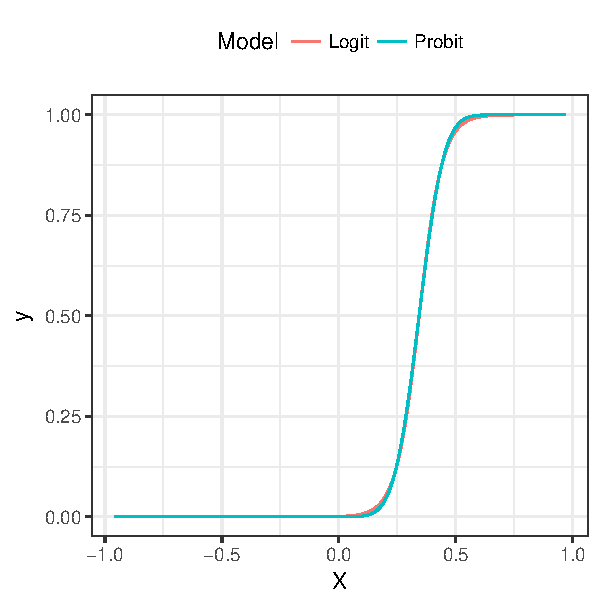
\includegraphics[width=\linewidth]{Probit-Logit-Fitted.pdf}
	\caption{Comparison of Probit and Logit Curves}
	\label{fig:Probit-Logit-Fit}
\end{figure}

Each of the estimation models was able to successfully select its own data generation process the majority of the time. The average model selection probability of the probit model under the probit data generation process was 0.679, and the probit marginal likelihood exceeded the logit marginal likelihood 96\% of the time in that case. Conversely, the average model selection probability of the logit model under the logit data generation process was 0.541, and the logit was more likely than the probit in 67\% of the simulations. While this result may initially seem underwhelming, it is made more impressive the remarkable similarity in probit and logit curves, as shown in \Cref{fig:Probit-Logit-Fit}.\footnote{These curves were produced using maximum likelihood estimates for each model against simulated data to illustrate similarities of the two curves in practical empirical modeling.}  Further, as mentioned in the previous subsection, model comparison between logit and probit models has presented a struggle for both classical and Bayesian methods. As shown in this example, iterative KDE (in addition to Laplace's method, bridge sampling, and similar methods where appropriate) opens the possibility of comparing these models in a statistically meaningful way.

\section{Parametric and Non-Parametric Stochastic Frontiers}

\label{sec:SF}

For each of the examples in the previous section, marginal likelihood could be consistently estimated using previously established methods, whether it be using methods from \cite{Chib} or \cite{ChibJeliazkov}, bridge sampling, Laplace's method, or similar techniques. However, as discussed in \cref{sec:ModelSelection}, existing techniques are not suitable for models that cannot be effectively estimated with Gibbs sampling or Metropolis-Hastings and have large numbers of parameters and moderate sample sizes. This section presents models and data for which iterative KDE is the only method that can reliably estimate marginal likelihood, to the best of my knowledge.

Stochastic frontier models, developed in the seminal paper \cite{AignerLovellSchmidt}, estimate production frontiers under an error specification with one- and two-sided components. Specifically, the model assumes output can be described by
\begin{equation}
	y_i = T(X_i) + \ep_i + \delta_i,
\end{equation}
where $y_i$ is the $i$th observation of log-output, $X_i$ are inputs, $T$ is some function that transforms inputs to outputs, $\ep_i$ is a two-sided error component (e.g., coming from a normal distribution), and $\delta_i$ is a negative one-sided error component (e.g., coming from a half-normal or exponential distribution). Estimation is possible when the density of the sum of one- and two-sided error components is specified. As detailed in \cite{AignerLovellSchmidt}, when $\ep\sim N(0, \sigma_\ep^2)$ and $\delta\sim N^-(0, \sigma_\delta^2)$, then the error term $v = \ep + \delta$ has the density function
\begin{equation}
	\label{eq:sfDensity}
	f_{NPHN}(v; \sigma_\ep, \sigma_\delta) = \frac2\sigma \phi\left(\frac{v}\sigma\right)\left(1 - \Phi\left(\frac{v\lambda}{\sigma}\right)\right),
\end{equation}
where $\sigma^2 = \sigma_\ep^2 + \sigma_\delta^2$, $\lambda = \sigma_\delta / \sigma_\ep$, and $\phi$ and $\Phi$ are standard normal density and distribution functions, respectively. The density function $f_{NPHN}$ represents a random variable which is the result of normal plus half-normal (NPHN) random variables, and we can write $V\sim NPHN(\sigma_\ep, \sigma_\delta)$ if $V$ follows the NPHN distribution with parameters $\sigma_\ep$ and $\sigma_\delta$.

Even with the exact form of the density function of the error composition, estimation of stochastic frontier models is notoriously difficult in a classical framework. Both maximum likelihood and method of moments routines suffer from numerical instability with these models, making it difficult to estimate parameters or even determine if those algorithms have properly converged. Estimating these models in a Bayesian framework using Markov Chain Monte Carlo reduces instability as even a weakly informative prior can help with model identification \citep{VanDenBroeck}.

Parametric specifications of $T$ have traditionally been used, typically in log-linear (each log-transformed input included) or translog (addition of all second-order log terms) form. Non-parametric forms of $T$ have also been recently proposed, such as in \cite{ParmeterRacine}, and typically involve a two-step procedure: First, the mean of the data is fit using some non-parametric method (such as kernel smoothing), then differences between the fitted curve and the observed data are assumed to be of the above form, from which parameters of the one- and two-sided distributions can be estimated. Unfortunately, this model cannot be used with likelihood-based model selection (and cannot even be estimated in a Bayesian framework) since the initial kernel smoothing step does not have an associated likelihood function. Cross-validation methods could be used, but as described in \cref{sec:ModelSelection}, those methods can be relatively data-intensive.

% latex table generated in R 3.5.0 by xtable 1.8-3 package
% Sun Oct 14 19:43:43 2018
\begin{table*}
\centering
\begin{tabular}{l|c|c|c}
  \multicolumn{1}{c}{} & \multicolumn{1}{c}{} & \multicolumn{1}{c}{Efficiency} & \multicolumn{1}{c}{} \\ 
   \cline{2-4}\multicolumn{1}{c}{Country} & \multicolumn{1}{c}{Log-linear} & \multicolumn{1}{c}{Translog} & \multicolumn{1}{c}{GP} \\ 
   \hline
\hline
Algeria & 0.865 & 0.787 & 0.77 \\ 
  Armenia & 0.775 & 0.732 & 0.75 \\ 
  Australia & 0.702 & 0.671 & 0.757 \\ 
  Azerbaijan & 0.832 & 0.777 & 0.786 \\ 
  Bulgaria & 0.81 & 0.816 & 0.775 \\ 
  China & 0.833 & 0.745 & 0.797 \\ 
  Croatia & 0.73 & 0.741 & 0.766 \\ 
  Cyprus & 0.709 & 0.655 & 0.753 \\ 
  Czech Republic & 0.805 & 0.76 & 0.781 \\ 
  Denmark & 0.887 & 0.853 & 0.838 \\ 
  Estonia & 0.763 & 0.793 & 0.789 \\ 
  France & 0.878 & 0.816 & 0.835 \\ 
  Hungary & 0.808 & 0.793 & 0.751 \\ 
  Jordan & 0.67 & 0.745 & 0.718 \\ 
  Latvia & 0.792 & 0.79 & 0.75 \\ 
  Libya & 0.735 & 0.704 & 0.743 \\ 
  Luxembourg & 0.795 & 0.698 & 0.744 \\ 
  Malta & 0.855 & 0.771 & 0.713 \\ 
  Mexico & 0.752 & 0.792 & 0.755 \\ 
  Netherlands & 0.875 & 0.798 & 0.79 \\ 
  Paraguay & 0.656 & 0.678 & 0.722 \\ 
  Poland & 0.768 & 0.736 & 0.752 \\ 
  Romania & 0.681 & 0.678 & 0.769 \\ 
  Serbia & 0.738 & 0.706 & 0.759 \\ 
  Slovak Republic & 0.759 & 0.729 & 0.724 \\ 
  Slovenia & 0.779 & 0.794 & 0.746 \\ 
  Spain & 0.727 & 0.779 & 0.744 \\ 
  Switzerland & 0.807 & 0.785 & 0.771 \\ 
  United Kingdom & 0.81 & 0.652 & 0.755 \\ 
   \hline
\end{tabular}
\caption{Mean Efficiency Estimates} 
\label{tab:EfficiencyEstimates}
\end{table*}


Gaussian processes (GPs) offer similar flexibility to kernel smoothing and can be estimated within a Bayesian framework \citep{Rasmussen}. Specifically, a typical GP model has the form
\begin{subequations}
\begin{align}
	\label{eq:GPBase:theta} \theta &\sim g_\theta(\phi_\theta)\\ 
	\label{eq:GPBase:sigma} \sigma &\sim g_\sigma(\phi_\sigma)\\ 
	\label{eq:GPBase:f} T(X) &\sim N(0, K_\theta(X))\\ 
	\label{eq:GPBase:y} y &\sim N(T(X), \sigma^2 I_N). 
\end{align}
\end{subequations}
\Cref{eq:GPBase:theta} and \cref{eq:GPBase:sigma} state the model parameters $\theta$ and $\sigma$ have priors of a form chosen by the researcher. \Cref{eq:GPBase:f} forms a prior over predicted values of $y$ given inputs $X$ and relates those predictions together with covariance kernel $K_\theta$. For a continuous kernel, this formulation assumes that the predicted production function is also continuous. A common choice for $K_\theta$ is the normal kernel, discussed in \cref{sec:KDE}. Finally, \cref{eq:GPBase:y} states that observations of $y$ have a mean of their predicted value, $T(X)$, and are conditionally independent with constant variance. Estimation of a GP yields an estimate for the entire function $T$, whose distribution (in the output space) can be calculated at any point in its domain \citep{RasmussenWilliams}. Since GPs can be estimated in a Bayesian framework, they can be candidates in Bayesian model selection. It is important to note that the flexibility offered by GPs is not without cost in model selection; each predicted value of $T(X)$ represents a parameter in the model. As discussed in \cref{sec:ModelSelection}, each additional parameter included in the model tends to reduce overall marginal likelihood if the parameter does not offer sufficient extra predictive power.

Given the large number of parameters in GP models, it can be difficult, if not impossible, to accurately perform model selection for moderately sized samples using any previously established method. If the sample size is not large, cross-validation may not be feasible and methods using asymptotic results may not be appropriate. Bayesian model selection may be suitable in theory, but given the large number of parameters, existing methods of estimating marginal likelihood for moderately-sized samples, such as bridge sampling, may not be reliable. Iterative kernel density estimation presents a technique for consistently estimating marginal likelihood in precisely this type of scenario.

The typical GP model presented above can easily be extended to represent a stochastic frontier. Specifically, rather than assuming the difference between observed and predicted output is normally distributed, one can assume observed errors follow the NPHN distribution, whose density was presented in \cref{eq:sfDensity}. This research utilizes the following model:
\begin{subequations}
\label{eq:GPSF}
\begin{align}
	\alpha&\sim \Gamma^{-1}(1, 1)\\
	H_{jj}&\sim \Gamma^{-1}(10, 1) \mbox{\ \ ;\ \ }j=1,...,k\\
	H_{jl} &= 0 \mbox{\hspace*{4.3em} ;\ \ }j\neq l\\
	\sigma_\ep &\sim \Gamma^{-1}(1, 1)\\
	\sigma_\delta &\sim \Gamma^{-1}(1, 1)\\
	T(X)&\sim N(0, K_{\alpha, H}(X))\\
	y - T(X)&\sim NPHN(\sigma_\ep, \sigma_\delta),
\end{align}
\end{subequations}
where $y$ is a $N\times 1$ vector of observations of log-output, $X$ is a $N\times k$ matrix of input observations, and $K_{\alpha, H}$ is a covariance matrix formed using the normal kernel, whose $jl$th element has the form
\begin{equation}
	\left(K_{\alpha, H}(X)\right)_{jl} = \alpha^2 \exp\left(X_j' H^{-1} X_l\right),
\end{equation}
where $X_j$ is the $j$th row of $X$. Priors were chosen to be relatively diffuse, with the exception of the priors on diagonal elements of the bandwidth matrix $H$, which were chosen so that the resulting GP would be flexible compared to log-linear and translog forms.

% latex table generated in R 3.5.0 by xtable 1.8-3 package
% Sun Oct 14 19:44:20 2018
\begin{table*}
\centering
\begin{tabular}{l|c|c|c|c|c}
   &  & Log & Log & Log & Log Marginal \\ 
  Model & \# Parameters & Likelihood & Prior & Posterior & Likelihood \\ 
   \hline
\hline
Log-Linear & 8 & -3.734 & -10.225 & 15.249 & -29.208 \\ 
  Translog & 23 & -0.699 & -23.666 & 44.62 & -68.984 \\ 
  GP & 37 & 2.68 & -27.937 & 21.458 & -46.716 \\ 
   \hline
\end{tabular}
\caption{Marginal Likelihood Estimates} 
\label{tab:GPSF-ML}
\end{table*}


To exemplify the ability to select between parametric and non-parametric stochastic frontier models, this research uses data describing cereal production in a variety of countries, made available by the World Bank \citep{WorldBank}. Specifically, the data include observations of 29 countries in 2012, using metric tons of cereal produced as the output variable, and five input variables: area of land used for cereal production, total fertilizer consumption, total withdrawals of fresh water used for agriculture, average rainfall, and total number of people working in agriculture. These were used to estimate log-linear, translog, and GP stochastic frontier models. The priors used for the GP stochastic frontier model are exactly as shown in \cref{eq:GPSF}. For log-linear and translog models, constant terms were assumed to have a prior distribution of $N(0, 10)$, slope coefficients had prior distribution $N(0, 1)$, and $\sigma_\ep$ and $\sigma_\delta$ each had prior distribution $\Gamma^{-1}(1, 1)$. Mean efficiency estimates for each model and country are shown in \cref{tab:EfficiencyEstimates}.

Marginal likelihoods were calculated for each model using iterative kernel density estimation. Results are shown in \cref{tab:GPSF-ML}, along with numbers of parameters, log-likelihood, log prior, and log posterior densities at mean parameter estimates for each model. As expected, more flexible models result in higher log-likelihood. However, the benefits of predictive power are largely outweighed by penalties from the inclusion of additional parameters, as seen by the log-linear model having the highest marginal likelihood. The GP stochastic frontier model presented the second best fit despite having more parameters than the translog; not only did the GP model have better predictive power (as evidenced by higher log-likelihood), but the parameters also served less redundant purposes (as shown by its lower log posterior). While the most parsimonious model performed best in this example, there are no doubt situations involving more complex relationships between inputs and outputs where benefits of additional flexibility in the functional form outweigh penalties.

\section{Conclusion}

Bayesian model selection can be used to compare very general classes of models even when data are limited. However, computation of model probabilities used in Bayesian model selection can be hard, and a number of methods have been developed to make the problem computationally feasible. While existing methods are well-suited to many models and data, there is not, to my knowledge, a technique that performs well for models with many parameters applied to relatively small datasets. This research develops a method of estimating marginal likelihood using iterative kernel density estimation (KDE) that performs well in such scenarios and in general. Simulation results show iterative KDE produces estimates of marginal likelihood that are unbiased, potentially more efficient than other methods, such as those presented in \cite{Chib}, and applicable to many types of models and data. An application of iterative KDE to a flexible stochastic frontier model indicates the method shows promise in evaluating complex models applied to relatively limited data.

\bibliographystyle{chicago}
\bibliography{Iterative_ML}

\end{document}
